\documentclass{beamer}
\usepackage[utf8x]{inputenc}
\usepackage[frenchb]{babel}
\usepackage{hyperref}
\usepackage[footheight=1em]{beamerthemeboxes}
\usepackage{listings}
\usepackage{ulem}
\usepackage{color}
%\usepackage{pgfpages}
%\setbeameroption{show notes on second screen=left}
\usetheme{Singapore}


\setbeamertemplate{footline}{
\leavevmode%
\hbox{
\hspace*{-0.06cm}
\begin{beamercolorbox}[wd=.8\paperwidth,dp=1ex,left]{section in head/foot}%
	\usebeamerfont{section in head/foot}
\end{beamercolorbox}%
\begin{beamercolorbox}[wd=.2\paperwidth,ht=2.25ex,dp=1ex,right]{section in head/foot}%
	\insertframenumber{}\hspace*{2ex}
\end{beamercolorbox}}%
\vskip0pt%
}

\setbeamertemplate{navigation symbols}{}

%\usetheme{Frankfurt}


%\addfootboxtemplate{\color{white}}{\color{gray}
  %\insertframenumber/\inserttotalframenumber\null}



\setbeamertemplate{background canvas}{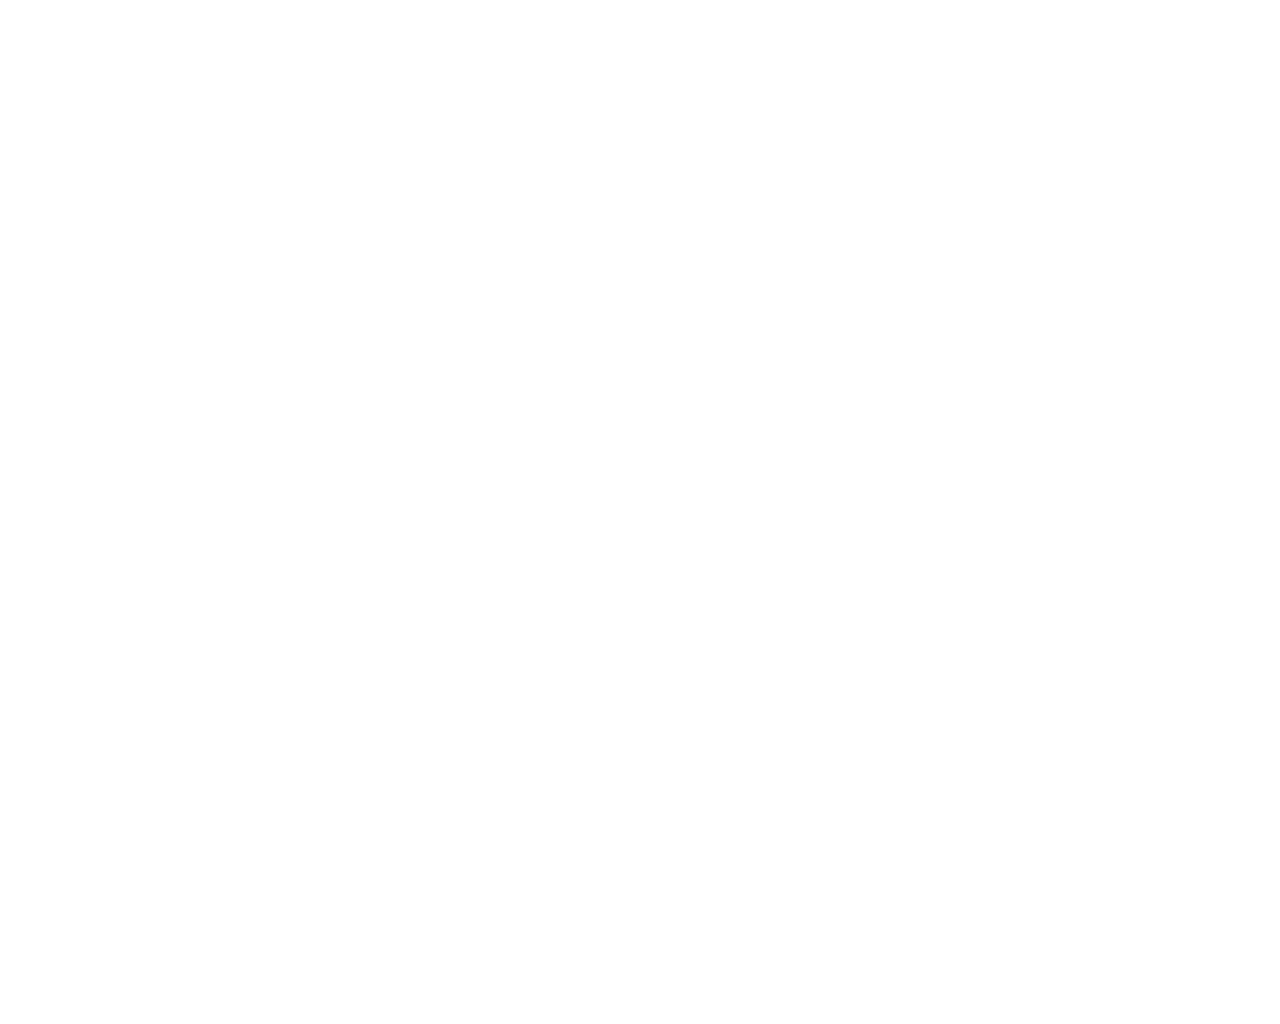
\includegraphics
   [width=\paperwidth,height=\paperheight]{files/fond.png}}


\title{HamSpamGram}
\author{Thibaut \textsc{Marmin} \and Namrata \textsc{Patel} \\ Clément \textsc{Sipieter}}
\institute{TP WEKA : fouille de données basée sur un corpus de SMS Spam.\\\texttt{https ://github.com/sipi/HamSpamGram}}
\date{24 Mai 2012}

\begin{document}

% Def variable coloration code source
\definecolor{keyword}{rgb}{0.55,0,0} 
\definecolor{type}{rgb}{0,0.55,0} 
\definecolor{comment}{rgb}{0.7,0.7,0.7} 

\lstset{
basicstyle=\footnotesize\sffamily,
numbers=none,
numberstyle=\footnotesize\color{comment},
keywordstyle=\color{keyword}\bfseries,
commentstyle=\color{comment},
breaklines=true,
fontadjust=true,
columns=fullflexible,
morekeywords=true
}

\AtBeginSection[]
{
  \begin{frame}{HamSpamGram}
  \begin{columns}[t]
  \begin{column}{5cm}
  \tableofcontents[sections={1-3},currentsection,hideothersubsections]
  \end{column}
  \begin{column}{5cm}
  \tableofcontents[sections={4-6},currentsection,hideothersubsections]
  \end{column}
  \end{columns}
  \end{frame}
}

\begin{frame}
\titlepage
\end{frame}

\begin{frame}{HamSpamGram}
    

  \begin{columns}[t]
  \begin{column}{5cm}
  \tableofcontents[sections={1-3},hideallsubsections]
  \end{column}
  \begin{column}{5cm}
  \tableofcontents[sections={4-6},hideallsubsections]
  \end{column}
  \end{columns}

\end{frame}

\section{Choix du corpus}
\subsection{Contraintes}
\begin{frame}{Choix du corpus}{Contraintes}
\begin{block}{Contraintes exprimées}
	\begin{itemize}
	\item Au moins deux classes
	\item Au moins 25 documents par classe
	\item Langue du corpus au choix
	\end{itemize}
\end{block}
\pause
\begin{block}{Contraintes implicites}
	\begin{itemize}
	\item Capacité à former le corpus
	\item Au moins deux classes \textbf{claires}
	\end{itemize}
\end{block}
\end{frame}

\subsection{Pistes}
\begin{frame}{Choix du corpus}{Pistes}
\begin{block}{Idées de corpus}
\begin{center}
	\begin{tabular}{|r c l|}
	\hline
	Œuvres Shakespeare & $\leftrightarrow$ & Œuvres Shakespeare \\
	\textit{Poésie} & & \textit{Théâtre} \\
	\hline
	Sites sains & $\leftrightarrow$ & Sites pornographiques \\
	\hline
	Unes du Monde & $\leftrightarrow$ & Unes du Monde \\
	\textit{Bonnes nouvelles} & & \textit{Mauvaises nouvelles} \\
	\hline
	Synopsis de films & $\leftrightarrow$ & Synopsis de films \\	
	\hline
	SMS Spams & $\leftrightarrow$ & SMS Légitimes \\	
	\hline
	\end{tabular}
\end{center}
\end{block}
\pause
\begin{block}{Notre choix}
Corpus \texttt{SMS Spam Corpus v.1} $\Rightarrow$ \nombre{5574} SMS dont
		\begin{itemize}
			\item \nombre{747} Spam
			\item \nombre{4827} Ham
		\end{itemize}
\end{block}
\end{frame}

\begin{frame}[containsverbatim]{Choix du corpus}{Pistes}
\begin{block}{Format des données}
\begin{verbatim}
ham   What you doing?how are you?
ham   Ok lar... Joking wif u oni...
spam  Sunshine Quiz! Win a super Sony DVD recorder if you canname the capital of Australia? Text MQUIZ to 82277. B
spam  URGENT! Your Mobile No 07808726822 was awarded a L2,000 Bonus Caller Prize on 02/09/03! This is our 2nd attempt to contact YOU! Call 0871-872-9758 BOX95QU
\end{verbatim}
\end{block}
\end{frame}

\section{Représentation des données}
\subsection{Stemmatisation}
\begin{frame}{Représentation des données}{Stemmatisation}
\begin{tabular}{l l l l}
\texttt{NLPToolkit} $\Rightarrow$ & \textbf{Porter}	& \textbf{Snowball}	& \textbf{Lancaster} \\
\hline
\uncover<2->{Mot 'win'}		& \uncover<2->{'win'}	& \uncover<2->{'win'}	& \uncover<2->{'win'} \\
\uncover<2->{Mot 'winner'}	& \uncover<2->{'winner'}& \uncover<2->{'winner'}& \uncover<2->{'win'} \\
\uncover<2->{Mot 'wing'}	& \uncover<2->{'wing'}	& \uncover<2->{'wing'}	& \uncover<2->{'wing'} \\

\hline
\uncover<3->{Mot 'react'}		& \uncover<3->{'react'}		& \uncover<3->{'react'}		& \uncover<3->{'react'} \\
\uncover<3->{Mot 'reacts'}		& \uncover<3->{'react'}		& \uncover<3->{'react'}		& \uncover<3->{'react'} \\
\uncover<3->{Mot 'reacting'}	& \uncover<3->{'react'}		& \uncover<3->{'react'}		& \uncover<3->{'react'} \\
\uncover<3->{Mot 'reaction'}	& \uncover<3->{'reaction'}	& \uncover<3->{'reaction'}	& \uncover<3->{'react'} \\
\uncover<3->{Mot 'reactions'}	& \uncover<3->{'reaction'}	& \uncover<3->{'reaction'}	& \uncover<3->{'react'} \\
\uncover<3->{Mot 'reactive'}	& \uncover<3->{'reactiv'}	& \uncover<3->{'reactiv'}	& \uncover<3->{'react'} \\
\uncover<3->{Mot 'reactivity'}	& \uncover<3->{'reactiv'}	& \uncover<3->{'reactiv'}	& \uncover<3->{'react'} \\
\uncover<3->{Mot 'reactant'}	& \uncover<3->{'reactant'}	& \uncover<3->{'reactant'}	& \uncover<3->{'react'} \\


\hline
\hline

\uncover<4->{Stats corpus} 	& \uncover<4->{2931}& \uncover<4->{2932}& \uncover<4->{2878} \\

\end{tabular}
\end{frame}

\subsection{Conversion $\Rightarrow$ \texttt{arff}}
\begin{frame}[containsverbatim]{Représentation des données}{Conversion $\Rightarrow$ \texttt{arff}}
\begin{block}{}
	\begin{itemize}
		\item Modèle booléen
		\item Modèle fréquentiste (TF)
		\item Modèle TF-IDF
	\end{itemize}
\end{block}
\begin{block}{}
\scriptsize
\begin{tabular}{|l|l|l|c|}
\hline
\textbf{Type} & \textbf{Préfixe} & \textbf{Contenu} & \textbf{Exemples} \\
\hline
\textit{Mot} & \verb+w_+ & La chaîne de caractère & \begin{minipage}{2cm}
\begin{verbatim}

w_bonjour
w_vive
w_le
w_master
w_decol

\end{verbatim}
\end{minipage} \\
\hline
\textit{Carac. Spécial} & \verb+c_+ & \begin{minipage}{4.5cm}\begin{displaymath}\begin{cases}
      \textrm{Code ASCII si ponctuation} \\
      \textrm{Caractère sinon}
\end{cases}
\end{displaymath} 
\end{minipage} & \begin{minipage}{2cm}
\begin{verbatim}

c_58
c_45
c_41
c_£

\end{verbatim}
\end{minipage} \\
\hline
\end{tabular}
\end{block}
\end{frame}

\section{Classification -- Sélection attributs}
\begin{frame} {Sélection d'attributs}
	\begin{itemize}
		\item Déterminer un sous-ensemble d'attributs pertinents 
		\pause
		\itemÉtude préalable sur corpus léger : 322 SPAM + 1002 HAM
		\pause
		\item Tests sur méthodes de recherche + méthode d'évaluation
	\end{itemize}
\end{frame}

\subsection{Etude préalable}
\begin{frame} {Etude préalable}{Tests}
	\begin{itemize}
		\item BestFirst+ CfsSubsetEval
		\pause
		\item GreedyStepwise + CfsSubsetEval
		\pause
		\item LinearForwardSelection+ CfsSubsetEval
		\pause
		\item Ranker + InfoGainAttributeEval
	\end{itemize}
\end{frame}

\begin{frame} {Etude préalable}{Test 1 : BestFirst + CfsSubsetEval}
\textbf{Paramètres :}
	\begin{center}
		\begin{tabular}{l cc}
			\textbf{direction} & Forward \\
			\textbf{startSet} & (vide) \\
		\end{tabular}
	\end{center}
\end{frame}

\begin{frame}{Etude préalable} {Test 2 : GreedyStepwise + CfsSubsetEval}
\textbf{Paramètres :}
	\begin{center}
		\begin{tabular} {l cc}
				\textbf{generateRanking} & False \\
				\textbf{searchBackwards} & False \\
				\textbf{startSet} & (vide)\\
		\end{tabular}
	\end{center}
\end{frame}

\begin{frame}{Etude préalable} {Test 3 : LinearForwardSelection + CfsSubsetEval}
\textbf{Paramètres :}
	\begin{center}
		\begin{tabular} {l cc}
			\textbf{forwardSelectionMethod} & False \\
			\textbf{numUsedAttributes} & False \\
			\textbf{performRanking} & True \\
			\textbf{startSet} & (vide) \\
		\end{tabular}	
	\end{center}
\end{frame}

\begin{frame}{Etude préalable} {Test 4 : Ranker + InfoGainAttributeEval}
\textbf{Paramètres : Variation du seuil}
	\begin{center}
		\begin{tabular}{c c}
			\textbf{threshold} & \textbf{Nb attributs}\\
			\nombre{0.005} & 356\\
			\nombre{0.01} & 184\\
			\nombre{0.02} & 90\\
			\nombre{0.03} & 57\\
			\nombre{0.04} & 37\\
			\nombre{0.05} & 30\\
		\end{tabular}
	\end{center}
\end{frame}

\subsection{Discussion}
\begin {frame}{Étude préalable} {Discussion}
Deux ensembles d'attributs distincts : 
	\begin{itemize}
		\item celui généré par les algorithmes utilisant la méthode d'évaluation \texttt{CfsSubsetEval}
		\item celui généré par les algorithmes utilisant la méthode d'évaluation \texttt{InfoGainAttributeEval}
	\end{itemize}
\end{frame}

\subsection{Nos choix}
\begin {frame} {Nos choix}
	\begin{itemize}
		\item \sout{BestFirst+ CfsSubsetEval}
		\item \textbf{GreedyStepwise + CfsSubsetEval}
		\item \sout{LinearForwardSelection+ CfsSubsetEval}
		\item \textbf{Ranker + InfoGainAttributeEval} en faisant varier le paramètre \og threshold \fg{}.
	\end{itemize}
\end{frame}

\section{Classification -- Méthodes}
\subsection{Choix des algorithmes}
\begin{frame}
  \begin{block}{Choix des algorithmes}
    \begin{itemize}
    \item J48
    \item NaiveBayes
    \item NBTree
    \item KStar
    \end{itemize}
  \end{block}
\end{frame}

\subsection{Mise en oeuvre}
\begin{frame}{Méthodes de classification}{Mise en oeuvre}
  \lstinputlisting[language=bash]{files/script.sh}
\end{frame}

\subsection{Résultats}
\begin{frame}{Méthodes de classification}{Résultats}

  Résultats par alghorithme de classification

  \begin{center}
    \scriptsize
    \begin{tabular}{l cccc} 
      \hline
      \textbf{Algorithme} & \textbf{Taux d'erreur} & \textbf{Précision*} & \textbf{Rappel*} & \textbf{F-mesure*}\\
      \hline
      J48 & 2.24 & 0.977 & 0.978 & 0.977\\
      KStar & 3.21 & 0.969 & 0.968 & 0.966\\
      NaivesBayes & 1.56 & 0.984 & 0.984 & 0.984\\
      NBTree & 1.35 & 0.987 & 0.987 & 0.986\\
    \end{tabular}
  \end{center}    
    \scriptsize\textbf{*}\textit{Moyenne pondérée}

\end{frame}


\begin{frame}{Méthodes de classification}{Résultats}
  
  Résultats par type de représentation des données
  
  \begin{center}
    \scriptsize
    \begin{tabular}{l cccc} 
      \hline
      \textbf{Modèle} & \textbf{Taux d'erreur}& \textbf{Précision*} & \textbf{Rappel*} & \textbf{F-mesure*}\\
      \hline
      Boolean & 1.35 & 0.987 & 0.987 & 0.986\\
      TF      & 1.56 & 0.984 & 0.984 & 0.984\\
      TFIDF   & 1.56\\
    \end{tabular}
  \end{center}    
    \scriptsize\textbf{*}\textit{Moyenne pondérée}

  
\end{frame}


\section{Règles d'association}
\subsection{Extraction de règles sur le corpus complet}

\begin{frame}[containsverbatim]{Règles d'association}{Extraction de règles sur le corpus complet}
\scriptsize
\begin{verbatim}
1. w_i=t c_39=t (897) ==> CLASS=HAM (883)        conf:(0.98)
2. w_my=t (613) ==> CLASS=HAM (602)              conf:(0.98)
3. w_i=t c_39=t c_46=t (584) ==> CLASS=HAM (570) conf:(0.98)
4. w_i=t (2084) ==> CLASS=HAM 2030               conf:(0.97)
5. w_i=t c_46=t (1450) ==> CLASS=HAM (1407)      conf:(0.97)
\end{verbatim}
\end{frame}

\subsection{Extraction de règles par classe}

\begin{frame}[containsverbatim]{Règles d'association}{Extraction de règles par classe}

\textbf{SPAM}
\scriptsize
\begin{verbatim}
6. c_46=t (589) ==> CLASS=SPAM (589)             
7. w_to=t (468) ==> CLASS=SPAM (468)             
8. c_46=t w_to=t (379) ==> CLASS=SPAM (379)      
9. c_33=t (366) ==> CLASS=SPAM (366)             
10. w_cal=t (322) ==> CLASS=SPAM (322)           
\end{verbatim}

\normalsize
\textbf{HAM}
\scriptsize
\begin{verbatim}
11. c_46=t (3080) ==> CLASS=HAM (3080)           
12. w_i=t (2030) ==> CLASS=HAM (2030)            
13. c_46=t w_i=t (1407) ==> CLASS=HAM (1407)     
14. w_you=t (1350) ==> CLASS=HAM (1350)          
15. c_39=t (1309) ==> CLASS=HAM (1309)           
\end{verbatim}

\end{frame}


\section{Clustering}
\begin{frame}{Clustering}{Modèle booléen}
\begin{center}
	\begin{tabular}{l||c|c}
	Cluster & \textbf{c0} (Ham) & \textbf{c1} (Spam)\\
	\hline
	\hline
	Spam & \nombre{652} & \nombre{95} \\
	\hline
	Ham & \nombre{3699} & \nombre{1128} \\
	\hline
	\% Spam & \nombre{18} & \nombre{8} \\
	\end{tabular}
\end{center}

$\Rightarrow$ Taux d'erreur : 30\%
\end{frame}

\begin{frame}{Clustering}{Modèle TF -- TF-IDF}

\begin{center}
	\begin{tabular}{l||c|c}
	Cluster & \textbf{c0} (Ham) & \textbf{c1} (noClass) \\
	\hline
	\hline
	Spam & \nombre{747} & \nombre{0} \\
	\hline
	Ham & \nombre{4806} & \nombre{21} \\
	\hline
	\% Spam & \nombre{16} & \nombre{0} \\
	\end{tabular}
\end{center}

$\Rightarrow$ Taux d'erreur : 14\%

\textit{Résultats identiques entre TF et TF-IDF}
\end{frame}

\end{document}
